\documentclass{beamer}

\usepackage[utf8]{inputenc}
\usepackage[spanish]{babel}
\usepackage{url}

% Más temas en
% http://deic.uab.es/~iblanes/beamer_gallery/index_by_theme.html
%\usetheme{Berlin}
%\usetheme{Copenhagen}
\usetheme{Warsaw}
%\usetheme{Darmstadt}

\setbeamercovered{transparent} %Items ocultos transparentes

\setbeamertemplate{background}{
  \rule{0pt}{.95\paperheight}%
  \hspace*{.98\paperwidth}%
  \makebox[0pt][r]{
\includegraphics[width=1.5cm]{fig/logo_fifa}}}

\title{Taller de Python}
\subtitle{Primer encuentro: Lo básico}
\author{FIFA}
\institute[FIFA]{Federación Interestudiantil de Física Argentina}
\date{\today}

%\AtBeginSubsection[]
%{
%  \begin{frame}<beamer>{Outline}
%    \tableofcontents[currentsection,currentsubsection]
%  \end{frame}
%}

% Let's get started
\begin{document}

\begin{frame}
  \titlepage
\end{frame}

%----------------------------------------------------------------------------------------------------------

\section{¿Qué es Python?}

\subsection{¿Qué es Python?}
\begin{frame}
    \frametitle{¿Qué es eso de Python? ¿Con qué se come?}
    Python es un \emph{lenguaje de programación}.\\ La \emph{única} forma de hablar con la computadora para que ella haga las cosas que nosotros queremos.
\end{frame}

\subsection{Instalación}
\begin{frame}
    \frametitle{Instalación de Python}
    \only<+>{Si tenés Linux, no prestes atención. Ya tenés instalado Python ;).}
    \begin{onlyenv}<+>
    Si tenés Windows, entrá en \url{www.python.org} y clickea en la pestaña Download, y luego en Windows. Ahí presioná la versión 2.7 (son muy parecidas, recomendamos usar la versión 3 para el futuro) y luego el archivo MSI installer (no el Program Database) correspondiente a 64 o 32bits, según el que tengas en tu sistema operativo (lo más usual es 64bits).
    \end{onlyenv}
\end{frame}



\begin{frame}
    \frametitle{Agregándole cosas a Python}
    A veces queremos hacer cosas que Python no sabe hacer, menos nosotros. Para eso otras personas en el mundo crearon \emph{paquetes}, que son programas organizados para fácil reutilización.
    
    Para instalar los paquetes, tenemos algunas opciones
    \begin{enumerate}
    \item{Instaladores, para Windows en \url{http://www.lfd.uci.edu/~gohlke/pythonlibs/}; y para Linux, dependiendo de la versión, hay que instalarlos de maneras diferentes.}
    \item{Con PIP, un programa escrito en Python que permite bajar las bibliotecas, en esta dirección \url{http://www.pip-installer.org}.}
    \item{Instalar un Python ''especial'', como Anaconda (\url{https://store.continuum.io/cshop/anaconda/}), que tiene un método especial para instalar los paquetes.}
    \end{enumerate}

\end{frame}

\begin{frame}
    \frametitle{Usando Python}
    Para este taller, vamos a usar el IDLE (Interactive Development Environment) llamado Spyder, un programa que nos ejecuta la consola de Python y nos permite escribir archivos .py desde el mismo lugar, con coloreado de palabras especiales y otros chiches. 
    
    La elección de este programa \emph{no} es única, y nosotros recomendamos usar el IPython, un paquete que agrega una consola interactiva muy parecida al Matlab/Octave/Mathematica. Además esta consola puede activar los paquetes de computación científica automáticamente. 
    
    Sin embargo el programa IDLE se instala \emph{por defecto} con Python

\end{frame}

%---------------------------------------------------------------------------------------------------------


\section{Nociones básicas de programación}

\subsection{¿Pero qué es hablar con la computadora?}
\begin{frame}
    \frametitle{¿Pero qué es hablar con la computadora?}
    La computadora ejecuta programas, que no son más que recetas:
    \begin{enumerate}
        \item Moje el cabello,
        \item Coloque champú,
        \item Masajee suavemente y deje actuar por 2 min.,
        \item Enjuague, y
        \item Repita el procedimiento (desde 1.-).
    \end{enumerate}
    
\end{frame}

\begin{frame}[fragile]
    Podemos ver que los pasos de toda receta sólo pueden hacer dos cosas:

    \begin{itemize}
        \item\uncover<1>{{\color{red} Transforman datos (o estados)}}
        \item\uncover<2>{{\color{blue} Cambian el flujo de las operaciones}}
    \end{itemize}
    \vskip 20pt
    \begin{enumerate}
        \item \uncover<1>{{\color{red}Moje el cabello}}.
        \item \uncover<1>{{\color{red}Coloque champú}},
        \item \uncover<1>{{\color{red}Masajee suavemente}} y \uncover<2>{{\color{blue}deje actuar por 2 min.}},
        \item \uncover<1>{{\color{red}Enjuague}}, y
        \item \uncover<2>{{\color{blue} Repita el procedimiento (desde 1.-)}}.
    \end{enumerate}
    
    
\end{frame}

\subsection{Nuestras herramientas hoy}
\begin{frame}[fragile]{Nuestras herramientas}

Utilizaremos Spyder como entorno para trabajar en Python. En las compus del laboratorio está disponible. Si trajiste tu compu, andá instalándotelo si no lo tenés.

\vskip11pt

Como guía de trabajo, utilizaremos la disponible en \emph{http://goo.gl/B2q73R}

\end{frame}



\subsection{¡Ahora sí! Empecemos con lo básico}
\begin{frame}[fragile]
  \frametitle{Empecemos con lo básico: las palabras}
  Como todo lenguaje, Python tiene un vocabulario de 31 palabras \emph{claves}
  \begin{verbatim}
    and       del       from      not       while
    as        elif      global    or        with
    assert    else      if        pass      yield
    break     except    import    print
    class     exec      in        raise
    continue  finally   is        return 
    def       for       lambda    try
  \end{verbatim}
  Con esto se puede hablar y escribir Python
\end{frame}

\subsection{¿Qué es un dato?}
\begin{frame}
    \frametitle{¿Qué es realmente un dato?}
    Los datos representan valores o cantidades de la vida real, como ser cantidad de manzanas que llevo en un canasto, o cantidad de monedas que puedo gastar al comprar un caramelo.
    \vskip11pt
    Un dato tiene un \emph{valor} numérico (binario), ya que la computadora debe guardarlo de alguna forma, pero si le defino un \emph{tipo} también se que es realmente y que representa de la vida real (un número, una palabra, etc).

\end{frame}

\begin{frame}
    \frametitle{¿Y qué tipo de datos puedo usar?}
    Los tipos de datos básicos son
    \begin{itemize}[<+->]
    \item Valores lógicos de verdad o valores \emph{booleanos} (\texttt{False} y \texttt{True})
    \item Enteros (1, 2, 5443, etc)
    \item Reales con punto decimal flotante (o coma flotante) (1.2, 5.61$\times 10^2$, etc)
    \item Cadenas (o \emph{strings}) de caracteres de texto (u'Hola Mundo',u"Ñoño'",u'\# Números' etc). Son un tipo especial de \emph{lista}, con métodos especiales.
    \item Listas de todos los anteriores sin necesidad de ser homogéneos ([1,2,3], ['H','o','l','a'], [True,False,0,1])
    \end{itemize}
\end{frame}

\begin{frame}[fragile]
    Ahora necesitamos las \emph{variables}. Escriban esto en la consola de Python
    \begin{verbatim}
        >>> a = 5
        >>> type(a)
        <class 'int'>
    \end{verbatim}
    Hicimos un entero, prueben con \texttt{True}, '5', 1.2 y [2, 3, 4]. \\Por ejemplo:
    \begin{verbatim}
        >>> a = '5'
        >>> type(a)
    \end{verbatim}
    %Nota: si vuelve a ejecutar \texttt{type(a)} sigue dando el último valor ingresado con \texttt{a = ALGO}. La operación \texttt{=} corresponde a \emph{asignar valores}, no igualdad.
\end{frame}

%----------------------------------------------------------------------------------------------------------

\section{Estructuras del lenguaje}
\subsection{Control de flujo}
\begin{frame}[fragile]
    \frametitle{Ahora un poco de control al asunto}
    Ejecuten el siguiente comando
    \begin{verbatim}
        >> print('Hola mundo')
        Hola mundo
    \end{verbatim}
    y ahora quiero repetirlo \textbf{10} veces. ¿Cómo lo hago?
    \begin{itemize}
    \item<+> Método mecánico \begin{verbatim}
     print('Hola mundo')
     print('Hola mundo')
     ...
     print('Hola mundo')
    \end{verbatim}
    \item<+> Que la computadora sepa que tiene que repetir 10 veces
    \end{itemize}
\end{frame}

\begin{frame}[fragile]
    \frametitle{El entorno $for$}
    ¿Cómo puede saber la computadora eso? Para eso existen bucles (loops en inglés). 
    \begin{verbatim}
    >>> for i in range(10):
    ...     print('Hola mundo')
    ...
    Hola mundo
    Hola mundo
    ...
    Hola mundo
    \end{verbatim}
    Ahora veamos qué es cada cosa\ldots
    
    \vspace{5mm}
    \tiny{Nota: \textbf{Acuérdense de revisar sintaxis y tabulado}}
\end{frame}
    
%\begin{frame}[fragile]
    

%\end{frame}

\begin{frame}[fragile]
\frametitle{El entorno $for$}
    \begin{onlyenv}<1>
        \begin{verbatim}
            >>> range(10)
            [0,1,2,3,4,5,6,7,8,9]
        \end{verbatim}
        Genera una lista del 0 a 9 (uno menos que el valor que ingresamos). \textbf{Tiene 10 elementos}.
        
        \vspace{2cm}
        \tiny{Nota: Prestar atención a que el primer elemento de las listas es el 0.
        Las listas tienen \textit{desde 0 hasta n-1 elementos}.
    \end{onlyenv}
    
    \begin{onlyenv}<2-3>
    Entonces con 
    \begin{verbatim}
        >>> for i in range(10):
        ...    print('Hola mundo')
        ...
    \end{verbatim}
    la computadora sabe \emph{literalmente} lo que dice, en inglés: por cada elemento \texttt{i} de la lista \texttt{range(10)}, haz \texttt{print('Hola mundo')}.

    \end{onlyenv}
    \only<3>{\center \alert{Es \emph{exactamente} lo que queríamos que la computadora hiciese}}
    \begin{onlyenv}<4>
        \vskip11pt
        Otro ejemplo, más ilustrativo de ''recorrer una lista''
        \begin{verbatim}
            >>> for i in range(10):
            ...     print(i)
            ...
            0
            1
            2
            ...
            9
        \end{verbatim}
    \end{onlyenv}

\end{frame}

\begin{frame}[fragile]
\frametitle{El entorno $for$}
    \frametitle{El entorno $while$}
    Además del \texttt{for}, existe otra estructura de bucle
    \begin{small}
    \begin{verbatim}
        >>> i = 0
        >>> while i < 10:
        ...     print(i)
        ...     i = i+1      -->  también pueden escribir
        ...                       i += 1 que es lo mismo
        0                         
        1
        ...
        9
    \end{verbatim}
    \end{small}
    El bucle al entrar verifica que \verb|i < 10| sea verdadero y luego ejecuta lo que viene abajo. Si no existiese el último comando \texttt{i = i+1}, nunca cambiaría el contador y nunca terminaría. Un bucle \emph{infinito}.
\end{frame}



\subsection{Condiciones en los programas}

\begin{frame}[fragile]
    \frametitle{Pongamos condiciones a este programa}
    ¿Qué pasa si tengo esto:
    \begin{verbatim}
        >>> for i in range(10):
        ...     print(i)
        ...
        0
        1
        2
        ...
        9
    \end{verbatim}
    pero quiero que imprima solamente los números pares entre 3 y 8 (inclusive), sin cambiar la lista que se ''recorre''? \footnotesize{(en general, no vas a poder hacer esto o no querés)}.
\end{frame}

\begin{frame}[fragile]
    \frametitle{El entorno $if$}
    \begin{onlyenv}<+>
    Para lo anterior tengo la siguiente estructura:
    \begin{verbatim}
    >>> for i in range(10):
    ...     if i <= 8 and i >= 3:
    ...         if i % 2 == 0:
    ...             print(i)
    ...
    \end{verbatim}
    El comando \texttt{if} ejecuta lo que viene a continuación sólo si la condición es verdadera (en este caso que \texttt{i} sea mayor que 3 y menor que 8). Las condiciones verdaderas dan valores booleanos \texttt{True}. 
    
    Vean que puedo tener \texttt{if} dentro de \texttt{if}, lo que se llama \textit{anidar}. 
    
    \vspace{5mm}
    \tiny{Nota: El comando \%, llamado \textit{módulo}, da el resto de la división de \texttt{i} en 2, que es 0 si \texttt{i} es par.}
    \end{onlyenv}
    
    
    \begin{onlyenv}<+>
        Prueben usar
        \begin{verbatim}
        >>> i = 3
        >>> i < 8
        True
        >>> i > 3
        False
        >>> i % 2 == 0
        False
        \end{verbatim}
        Para igualar expresiones en el sentido matemático usamos \texttt{==}.
    \end{onlyenv}
\end{frame}

\begin{frame}[fragile]
    \frametitle{El entorno $if$}
    \begin{onlyenv}<1-2>
    Resumiendo, el \texttt{if}
    \begin{verbatim}
    >>> if CONDICION:
    ...     ejecuto si es verdadero
    \end{verbatim}
    \end{onlyenv}
    \only<2>{¿Que pasa si quiero ejecutar algo si es falsa la condición?}
    \begin{onlyenv}<3>
        Agrego un \texttt{else}
        \begin{verbatim}
        >>> a = 3
        >>> if a < 5:
        ...     print(True)
        ... else:
        ...     print(False)
        ...
    \end{verbatim}
    \end{onlyenv}
    \begin{onlyenv}<4>
        Si no es verdadera la condición inicial, podemos preguntarnos si hay una condición que si sea verdadera, como en el caso anterior
        \begin{verbatim}
        >>> a = 3
        >>> if a < 5:
        ...     print(True)
        ... elif a == 5:
        ...     print('Iguales')
        ... else:
        ...     print(False)
        ...
    \end{verbatim}
    Primero verifica la primera, después verifica la segunda condición y si ninguna es verdadera ejecuta lo que está dentro de \texttt{else}.
    \end{onlyenv}
\end{frame}

\subsection{Funciones}

\begin{frame}[fragile]
    \frametitle{El entorno $if$}
    \frametitle{Reutilizando la receta}
    Imaginate que tenés que ejecutar una operación de forma seguida pero no de forma regular, como por ejemplo
    \begin{verbatim}
        >>> a = 2
        >>> b = 5
        >>> c = 3
        >>> d = a + b + c
        >>> d
        10
    \end{verbatim}
    
    
\end{frame}

\begin{frame}
\frametitle{Reutilizando la receta}
    Algo tan simple como eso lo queremos hacer modular, queremos una estructura que nos de posibilidad de sumar 3 números en cualquier lugar.\\
    \only<2->{\begin{center}¿Cómo lo hacemos?\end{center}}
    \only<3>{\huge\center Funciones}

\end{frame}

\begin{frame}[fragile]
\frametitle{Funciones}
    \begin{verbatim}
        >>> def Suma(a,b,c):
        ...     d = a + b + c
        ...     return d
        >>> Suma(2,5,3)
        10
    \end{verbatim}
    Prueben transformar en funciones todo lo que escribieron hasta ahora.
    
    \texttt{a,b,c} son \emph{argumentos} de la función Suma y con \texttt{return} la función devuelve un resultado, como una función matemática.
\end{frame}


\begin{frame}[fragile]
    \frametitle{Funciones que nos resuelven todo}
    ¿Se acuerdan de \texttt{range(10)}? Bueno, es una función de una biblioteca o \emph{biblioteca} básica de Python.
    
    Las funciones básicas más usadas
    {\small
    \begin{center}
    \begin{verbatim}
    abs()     bin()   bool()   chr()   
    divmod()  float() format() help()  
    input()   open()  print()  len()
    list()    map()   max()    min()   
    range()   type()     
    \end{verbatim}
    \end{center}
    }
    De las funciones básicas, la más importante para el recién empezado es la función \texttt{help()} a la cual le podemos pasar el nombre de cualquier función e imprimirá la ayuda escrita previamente. Por ejemplo, escriban \texttt{help(list)} (pueden salir presionando \emph{q})

\end{frame}

\begin{frame}[fragile]
    \frametitle{Más funciones que nos resuelven todo}
    En caso de querer usar funciones matemáticas necesitamos usar
    \begin{verbatim}
    >>> import math
    >>> math.sin(math.pi)
    -1
    \end{verbatim}
    Con \texttt{import} le decimos al intérprete de Python que traiga el paquete math y ahí vos lo podés usar.\\ Como ya vimos antes, los \emph{paquetes} son programas y utilidades organizadas para el uso posterior, en particular los programas están organizados en funciones ya que son \emph{el método} usado para reutilizar programas.
\end{frame}

\begin{frame}[fragile]
\frametitle{Más funciones que nos resuelven todo}
    Otro ejemplo puede ser el paquete \texttt{os}, que son funciones de sistema operativo
    \begin{verbatim}
    >>> import os
    >>> os.urandom(10)
    \end{verbatim}
    que nos da una cadena aleatoria de 10 bytes.

    Hasta ahora hablamos de paquetes básicos de la instalación. En próximos encuentros hablaremos profundamente de las bibliotecas científicas \textsc{numpy}, \textsc{scipy} y \textsc{matplotlib}, que pueden ir bajando e instalado.
\end{frame}


\begin{frame}[fragile]{Gráficos}

Trabajaremos con una de estas para graficar (\textsc{matplotlib})
y con otra para trabajar numéricamente (\textsc{numpy})
\begin{verbatim}
>>> from matplotlib import pyplot as plt
>>> import numpy as np
\end{verbatim}

Probaremos graficar una función elemental.
\end{frame}

\begin{frame}[fragile]

Inventemos un dominio y una función imagen. Son supuestas mediciones así que aportemos ruido.

\begin{verbatim}
>>> x = np.linspace(-5, 5)
>>> y = x**2 -3

>>> ruido = np.random.rand(len(y))*0.8
>>> y = y+ruido
\end{verbatim}
\end{frame}

\begin{frame}[fragile]

Ahora pidamos que grafique.

\begin{verbatim}
>>> plt.scatter(x, y)
>>> plt.xlabel('Variable independiente')
>>> plt.ylabel('x^2')
>>> plt.grid()

>>> plt.show() #(que nos muestre el gráfico)
\end{verbatim}
\end{frame}


\begin{frame}[fragile]

\begin{figure}
\centering
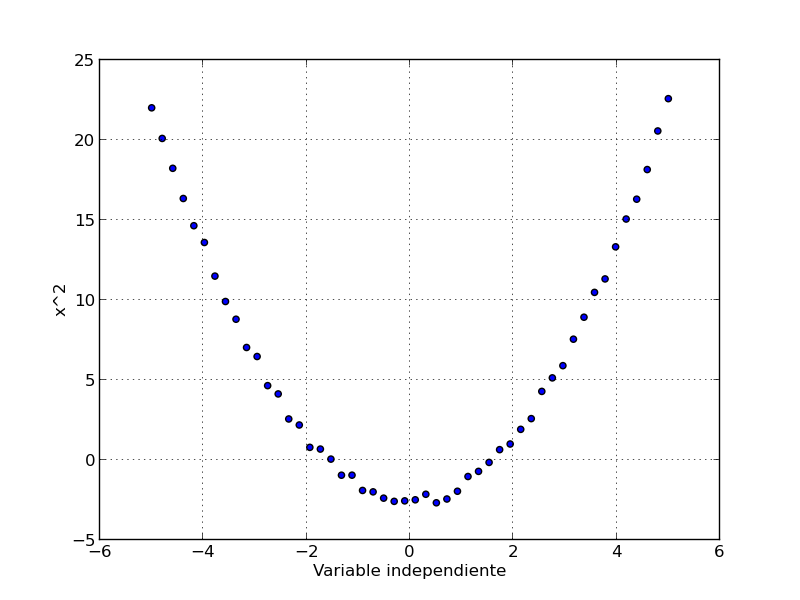
\includegraphics[width=0.8\textwidth]{fig/Grafico.png}
\caption{Gráfico de $f(x) = x^2-3$}
\label{fig:my_label}
\end{figure}

\end{frame}

%----------------------------------------------------------------------------------------------------------

\section{Para la próxima\ldots}

\subsection{Para seguir profundizando}
\begin{frame}
    \frametitle{Para seguir profundizando}
    Con esto vimos lo básico de programación en Python.\\
    Para seguir buscando tenemos\\
    \url{http://python.org.ar/}\\
    que tiene muchas páginas y libros para buscar. También recomendamos el tutorial en\\
    \url{http://www.learnpython.org}
    y el libro, con muchos ejemplos y exigiendo nada al lector:\\
    Lutz, M (2008). \emph{Learning Python}. 3era Ed. O'Really
\end{frame}


\subsection{En el próximo capítulo del Taller de Programación para laboratorio\ldots}
\begin{frame}
    \frametitle{Para la próxima}
   \begin{itemize}
   \item Ajustes lineales
   \item Interpolaciones
   \item Derivación numérica
   \item Integración numérica
   \item Estadística básica
   \end{itemize}
\end{frame}




%\begin{frame}{Blocks}
%\begin{block}{Block Title}
%You can also highlight sections of your presentation in a block, with it's own title
%\end{block}
%\begin{theorem}
%There are separate environments for theorems, examples, definitions and proofs.
%\end{theorem}
%\begin{example}
%Here is an example of an example block.
%\end{example}
%\end{frame}

% Placing a * after \section means it will not show in the
% outline or table of contents.
%\section*{Summary}

\begin{frame}
  
  \begin{center}\begin{Huge} ¡Gracias por venir! \end{Huge}\end{center}
\end{frame}



% All of the following is optional and typically not needed. 
%\appendix
%\section<presentation>*{\appendixname}
%\subsection<presentation>*{For Further Reading}

%\begin{frame}[allowframebreaks]
%  \frametitle<presentation>{For Further Reading}
    
%  \begin{thebibliography}{10}
    
%  \beamertemplatebookbibitems
  % Start with overview books.

%  \bibitem{Author1990}
%    A.~Author.
%    \newblock {\em Handbook of Everything}.
%    \newblock Some Press, 1990.
 
    
%  \beamertemplatearticlebibitems
  % Followed by interesting articles. Keep the list short. 

%  \bibitem{Someone2000}
%    S.~Someone.
%    \newblock On this and that.
%    \newblock {\em Journal of This and That}, 2(1):50--100,
%    2000.
%  \end{thebibliography}
%\end{frame}

\end{document}
